\documentclass[journal]{IEEEtran}

\usepackage{graphicx}
\usepackage{fancyhdr}
\usepackage{epsfig} % for postscript graphics files
\usepackage{graphics} % for pdf, bitmapped graphics files

\pagestyle{fancy}
\lhead{CPE 470/670}
\rhead{\thepage}
\chead{Team 6: Lab 4 Report}
\lfoot{}
\rfoot{}
\cfoot{}

\begin{document}

\begin{titlepage}
    \vspace*{\fill}
    \begin{center}
      {\LARGE \bf Lab 5: Line Following Robot}

      {Team 6: Alexander  C. Woods and Taylor Mansfield}

      October 15, 2014
    \end{center}
    \vspace*{\fill}
  \end{titlepage}


\section{Hardware and Software Design}\label{S.design}
\IEEEPARstart{L}{ine} following is a classic robotics problem and has been solved in a myriad of ways. The objective of this challenge is for the robot to follow a line as quickly as possible until it reaches the end, designated by a yellow square. Once at the end, the robot is to search for its home location, using sound information from the audience to guide it. The test environment includes a line which spirals in to a center point as shown in Fig. ~\ref{F.field}



\begin{figure}[h]
 \centering
  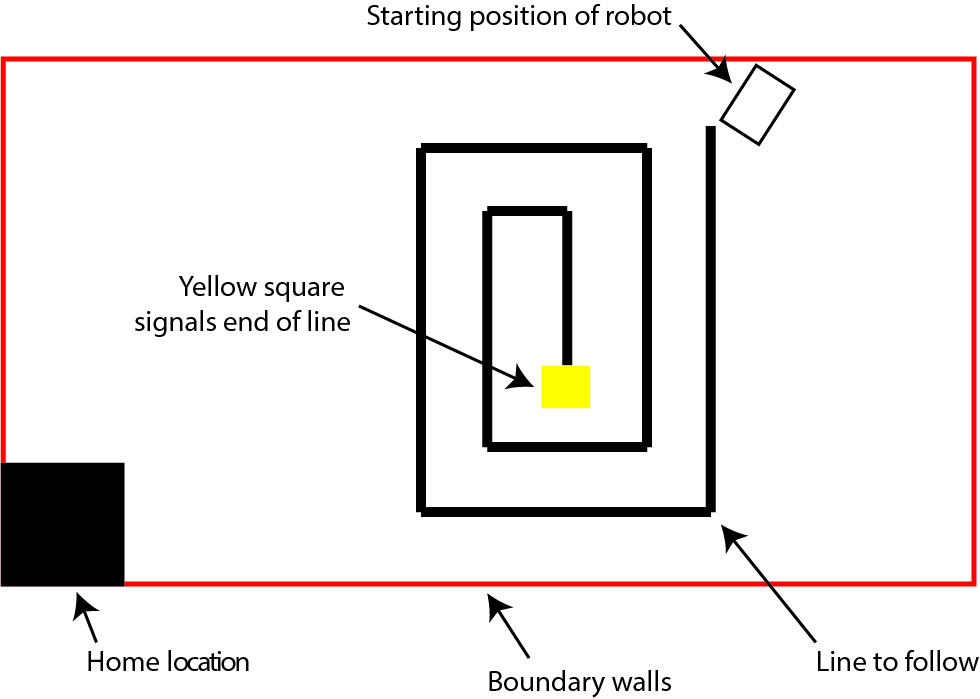
\includegraphics[width=1\columnwidth]{field.jpg}\\
  \caption{The test field was rectangular, with various food items spread throughout the area. A home area was marked by a black square in a corner of the field.}
  \label{F.field}
\end{figure}

The driving base for the food finding robot was the same as in previous labs, however the sensors and their locations were modified. The sonar sensors moved closer to the center of the robot to reduce blind spots and lowered in order to see the boundary walls. A light sensor and RFID sensor were mounted so that they would run over the various food as the robot searched.

The light sensor was mounted in such a way that the height could be adjusted so that it would give better readings. The mounted position could have been improved so that once set, the height did not change.

The software design of this robot consisted of two phases. The first phase is searching for food, and the second is finding the home location once the time had expired.

In the first phase, several tasks had to be managed simultaneously. The robot needed to execute a search pattern which would not repeat, had to monitor its surroundings for obstacles and walls, as well as monitors its color and RFID sensors for the presence of food.

The search behavior was developed such that the robot would continuously rebound off of walls when it approached them, but would also spin three times throughout the search in order to prevent a repetitive search pattern from developing. In testing and application, this method was effective.

The robot monitored for walls and obstacles much like it did in the previous corner escape contest. Using sonar sensors, the robot would veer away from walls that were within a close threshold, and would stop and turn away from walls that we within a very close threshold.

Monitoring for food consisted of checking the sensors in a loop, and playing a sound if a piece was found. For RFID tags, this was accomplished by monitoring the value of the sensor and playing a tone if it was anything other than zero, which is returned in the presence of no tags or cards. For color cards, if either the G or B values read were less than an experimentally determined threshold of 230 then there was a color present and the NXT would sound a tone.

Finally, when the time had expired our robot set a flag that time was up. This disabled all searching and gathering behavior and enabled the find home functionality. This function was designed such that the robot would find any wall, turn to the right, and proceed in a clockwise direction around the course until it sensed the black color of the home location. In order to avoid dragging along the wall during this process, the robot would bounce off the wall, and then curve back towards it in an arching pattern. This ensured that the robot did not hit the wall, but also never left it and got lost.

\section{Problems Encountered}\label{S.problems}
We encountered a few problems in both software and hardware design. In hardware, we quickly realized that it would be very difficult to navigate the field with only one sonar sensor to detect obstacles.

In software, we found that while using a multi-threaded software design allowed us to design individual behaviors that could cooperate with each other, the various functions could not be terminated on command after completing without additional firmware on the NXT. Additionally, the robot sometimes behaved in unexpected manners due to functions interfering with each other.

There also was a problem with how the robot navigated the field, that is, the search methodology. We found that a simple process of "bouncing" off of the walls of the field could cause a fixed pattern to develop where the robot would cover the same ground over and over again.

We also had severe problems with detecting the white background of the field reliably, as well as distinguishing the black go home area from the white background.

Lastly, our original "go home" strategy consisted of ramming into the wall at an angle and then hugging the wall until home was reached. This was always successful, but it would take a lot of time, especially when it began its search at a far corner of the field. Another approach using bumping would sometimes miss the home area by a small amount and have to loop again.

\section{Solutions}\label{S.solutions}
We decided to use dual sonar sensors at a slight angle like our previous design to overcome the navigation problem. Unlike our previous design, we put the two sonar sensors much closer together and lower to meet the level of the walls of the field. This eliminated the gap in ultrasonic "vision" at the front of the robot which would sometimes cause the robot to jam straight onto a wall and become stuck.

Going over the mutex handoffs allowed us to find spots where two threads could have control of the motor systems at the same time, or in rapid succession. Some restructuring of the tasks fixed the issue. In addition, we used a global bool variable to mark the mode of the robot in which certain tasks would fall out of their loops when the bool was changed so that the task did not need to be terminated manually.

In order to stop the search pattern from occasionally following the same path, we added a spinning task that would slightly alter the robot's orientation periodically to introduce randomness into the robot's path. This proved to be very successful at covering more area of the field quickly.

We had to play a lot with the mounted height of the color sensor in order to get a reliable reading. In addition, using the ReadSensorHTColor() function proved to give us much more reliable color readings with a finer grasp of the color makeup in RGB space.

Finally, by increasing the backward duration of the robot's left turn movement and introducing arching and right turn correction for the right sonic sensor, we were able to get the robot to get home within one lap around the field every time.

\section{Unsolved Problems}\label{S.unsolved}
During the competition, we scored almost no points for RFID detection, despite the RFID sensor going over the RFID tags several times. Especially for the smaller RFID tags, the RFID sensor seemed to have a very difficult issue with detecting tags. We believe this was due to the velocity of the robot, but it could also be due to power output from the RFID sensor or it's polling frequency or the proximity to the floor.

\end{document}
